\section{Evaluation}
\label{eval}

\subsection{YFCC100M Dataset}
\label{dataset}

Here goes an explanation of the dataset and all the source
(images, metadata, videos, features).

\subsection{Experimental Setup}

Here goes explanation of the comparison systems.
Need versions of MYSQL, OS, amount of memory and CPU info.

\begin{figure*}[]
\centering
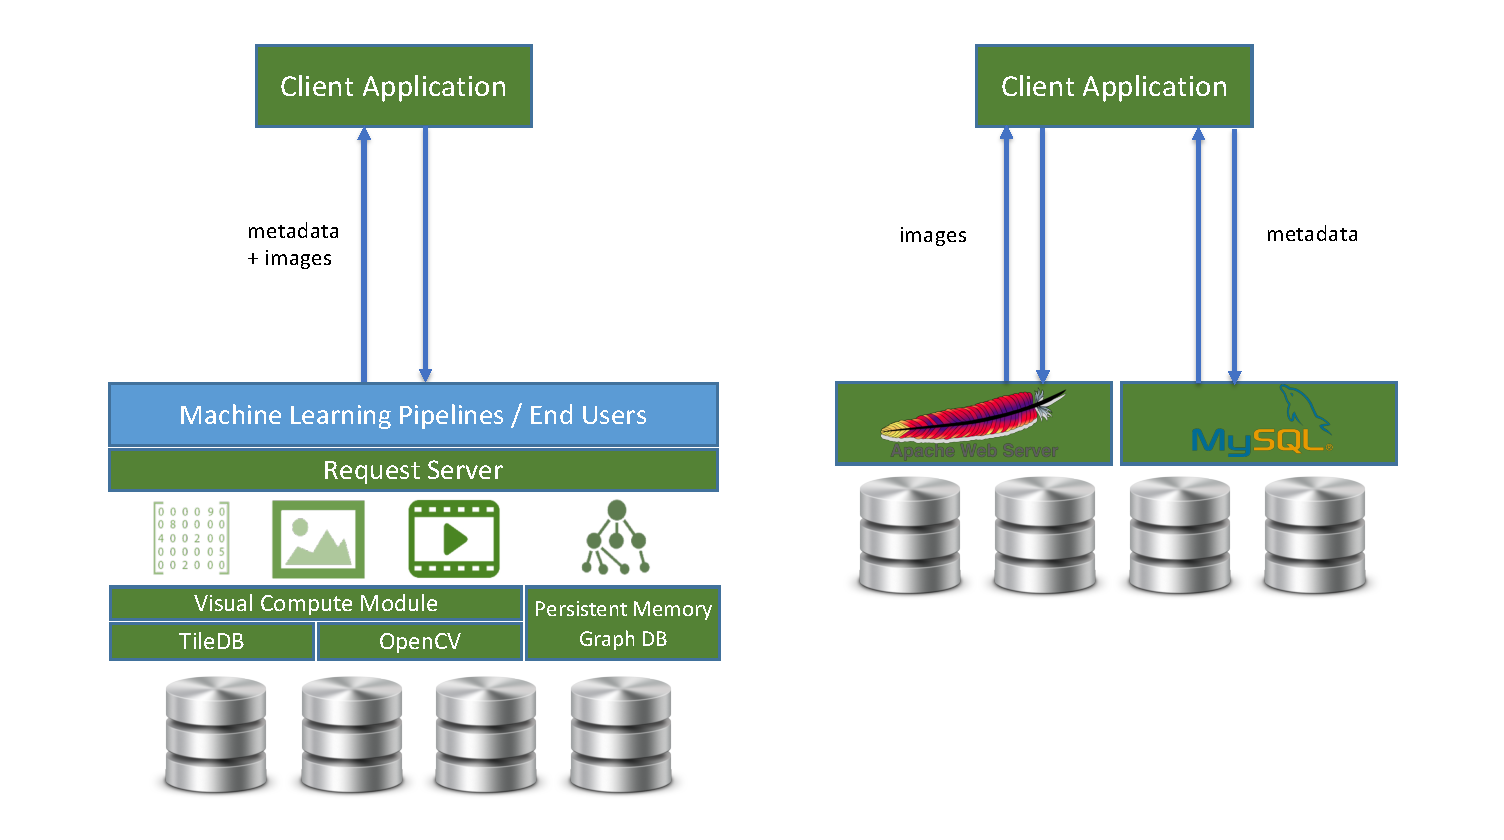
\includegraphics[width=\textwidth]{figures/comparison_system}
\caption{Comparison Systems}
\label{fig:systems}
\end{figure*}

\begin{table}[h]
\caption{Edges in VDMS database}
\centering
\begin{tabular}{c c c c}
\hline\hline
Database Size & No. Connections & MetaData & Tags\\
\hline
100k & 848,432 & 100,000 & 1,570\\
500k & 4,249,500 & 500,000 & 1,570\\
1M & 8,503,045 & 1,000,000 & 1,570\\
5M & 42,505,478 & 5,000,000 & 1,570\\
10M & 85,040,404 & 10,000,000 & 1,570\\
50M & 425,162,070 & 50,000,000 & 1,570\\
100M & 895,572,430 & 99,205,984 & 1,570\\
\hline
\end{tabular}
\label{table:vdmsedges}
\end{table}

The MySQL setup was implemented in a similar manner.  For each database, three tables were created: taglist, metadata, and autotags.  The taglist table contains the unique YFCC tags where each entry is given an integer index named tagid. The metadata table contains the YFCC metadata where the id column is used as the primary index. The autotags table contains the probabilities for the tags associated with the metadata entries of the metadata table using id and tagid as indices.  Each metadata entry has approximately nine tags; therefore, the number of rows in autotags is linearly related to the size of the MySQL database as shown in Table~\ref{table:mysqltables}.

\begin{table}[h]
\caption{Rows in MySQL database}
\centering
\begin{tabular}{c c c c}
\hline\hline
 & \multicolumn{3}{c}{Table}\\
\cline{2-4}
Database Size & Autotags & MetaData & Tag List\\
\hline
100k & 848,912 & 100,000 & 1,570\\
500k & 4,241,200 & 498,707 & 1,570\\
1M & 8,508,380 & 1,000,000 & 1,570\\
5M & 42,425,905 & 4,987,379 & 1,570\\
10M & 85,095,265 & 10,000,000 & 1,570\\
50M & 425,446,208 & 50,000,000 & 1,570\\
100M & 896,002,496 & 99,206,564 & 1,570\\
\hline
\end{tabular}
\label{table:mysqltables}
\end{table}

Table~\ref{table:metadata} compares the time to build and the size of the YFCC datasets as VDMS and MySQL databases.  On average, it takes MySQL 3.7x hours longer than VDMS to build the databases even though [insert relationship VDMS edges to mysql rows]. As a graph database, VDMS requires approximately 1.4x more storage than MySQL to store each database.

\begin{table*}[h]
\caption{Time (in hours) to build and size (in GB) of MySQL and VDMS databases}
\centering
\begin{tabular}{c c c c c}
\hline\hline
 & \multicolumn{2}{c}{Building Metadata Time} & \multicolumn{2}{c}{Metadata Size}\\
\cline{2-3} \cline{4-5}%\hline
Database Size & MySQL & VDMD & MySQL & VDMS\\
\hline
100k & 0.2 & 0.1 & 0.173 & 0.226\\
500k & 1.1 & 0.4 & 0.805 & 1.1\\
1M & 2.2 & 0.6 & 1.6 & 2.2\\
5M & 11.7 & 3.0 & 7.8 & 11\\
10M & 22.1 & 6.0 & 16 & 22\\
50M & 147.1 & 24.2 & 78 & 109\\
100M & 263.0 & 72.5 & 163 & 228\\
\hline
\end{tabular}
\label{table:metadata}
\end{table*}

\subsection{Images + Metadata}

Explanation of the evaluation and description of some of the queries.

\begin{figure}[]
\centering
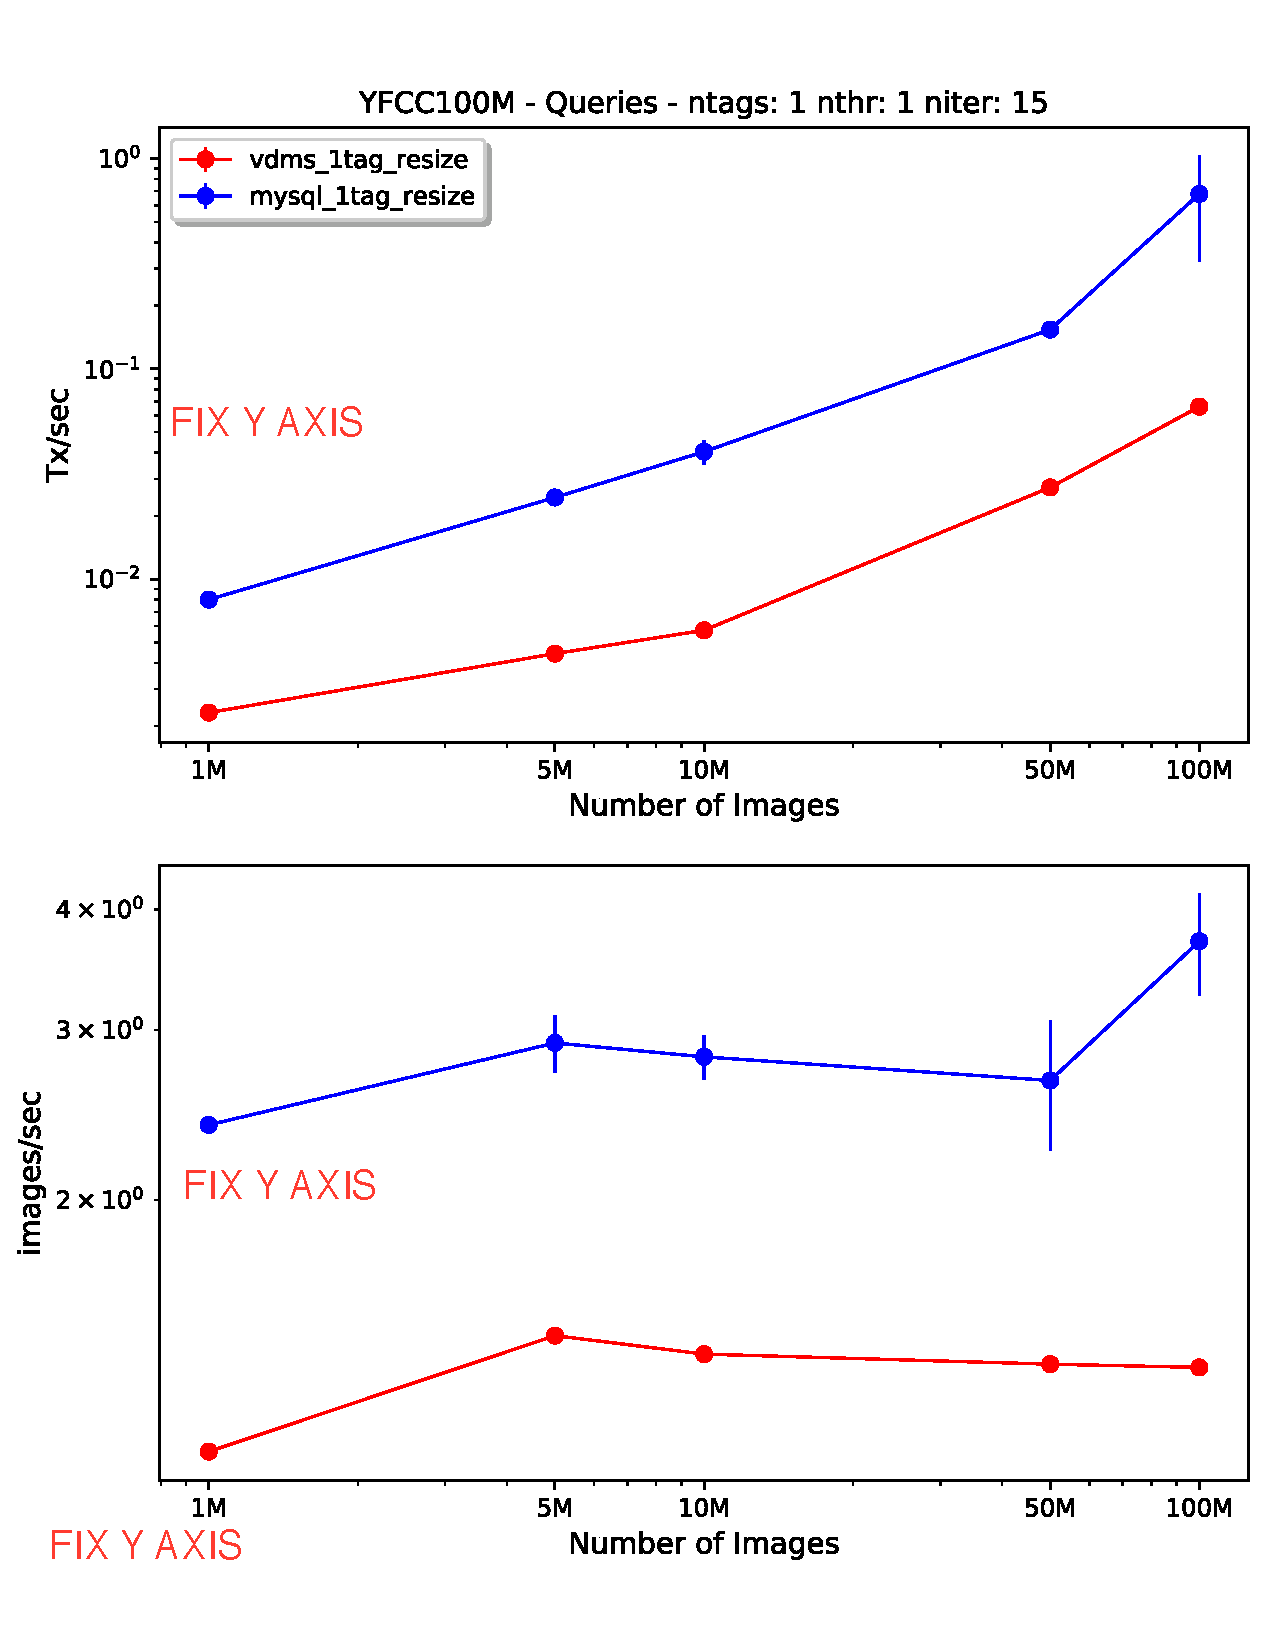
\includegraphics[width=\columnwidth]{figures/q1_latency}
\caption{Query 1 - Latency}
\label{fig:q1_latency}
\end{figure}

\begin{figure}[]
\centering
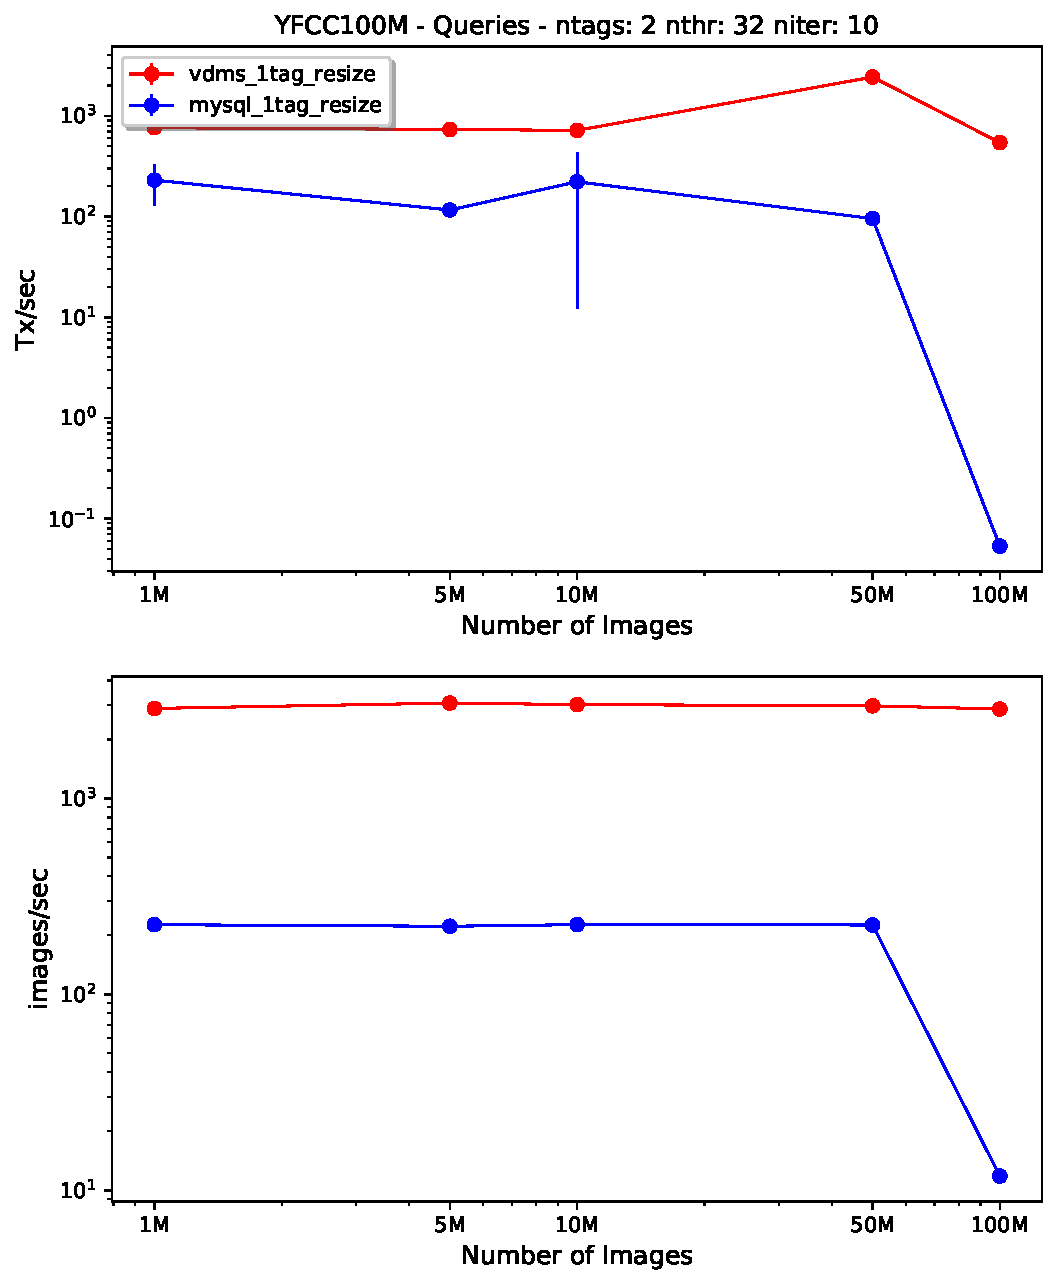
\includegraphics[width=\columnwidth]{figures/q1_throughput}
\caption{Query 1 - Throughput}
\label{fig:q1_throughput}
\end{figure}

\subsection{Videos}

Explanation of the video queries and comparison.
Explain concurrency.

\begin{figure*}[]
\centering
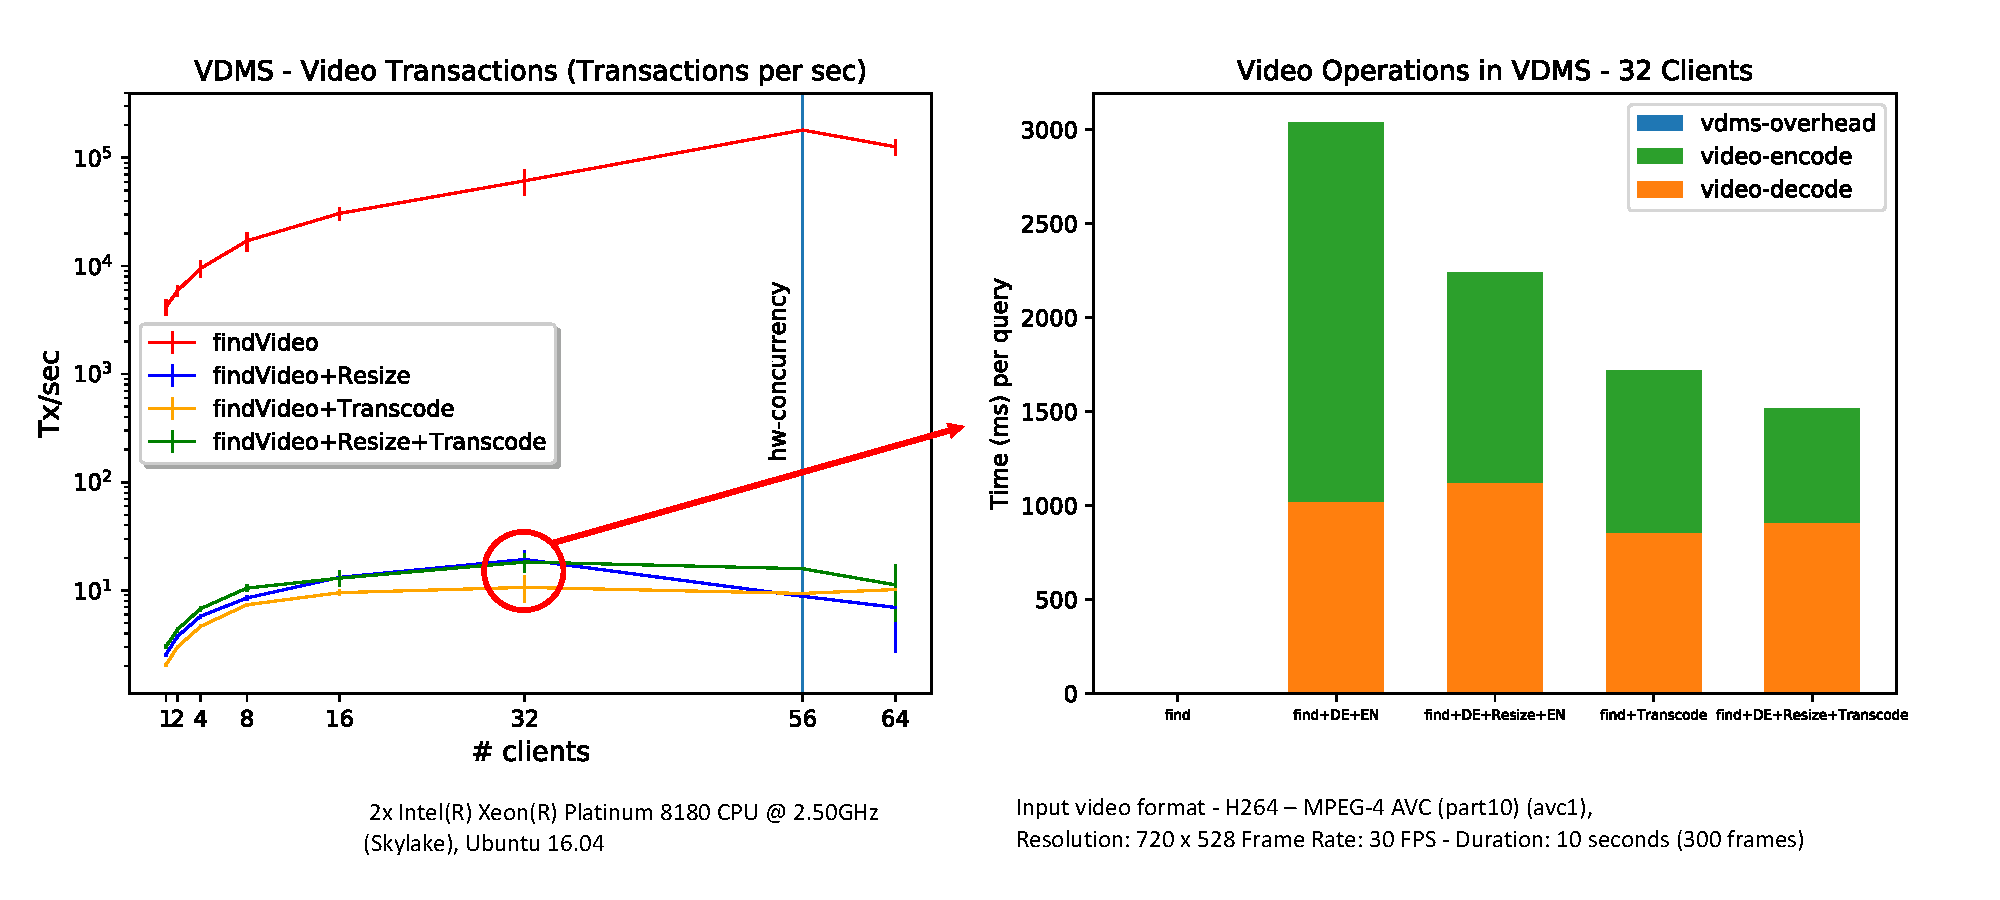
\includegraphics[width=\textwidth]{figures/video_overhead}
\caption{Concurrency and Overhead}
\label{fig:video}
\end{figure*}

\subsection{Feature Vectors}

Explain different engines supported, and how the features vectors
were ingested and handled.

\begin{figure*}[]
\centering
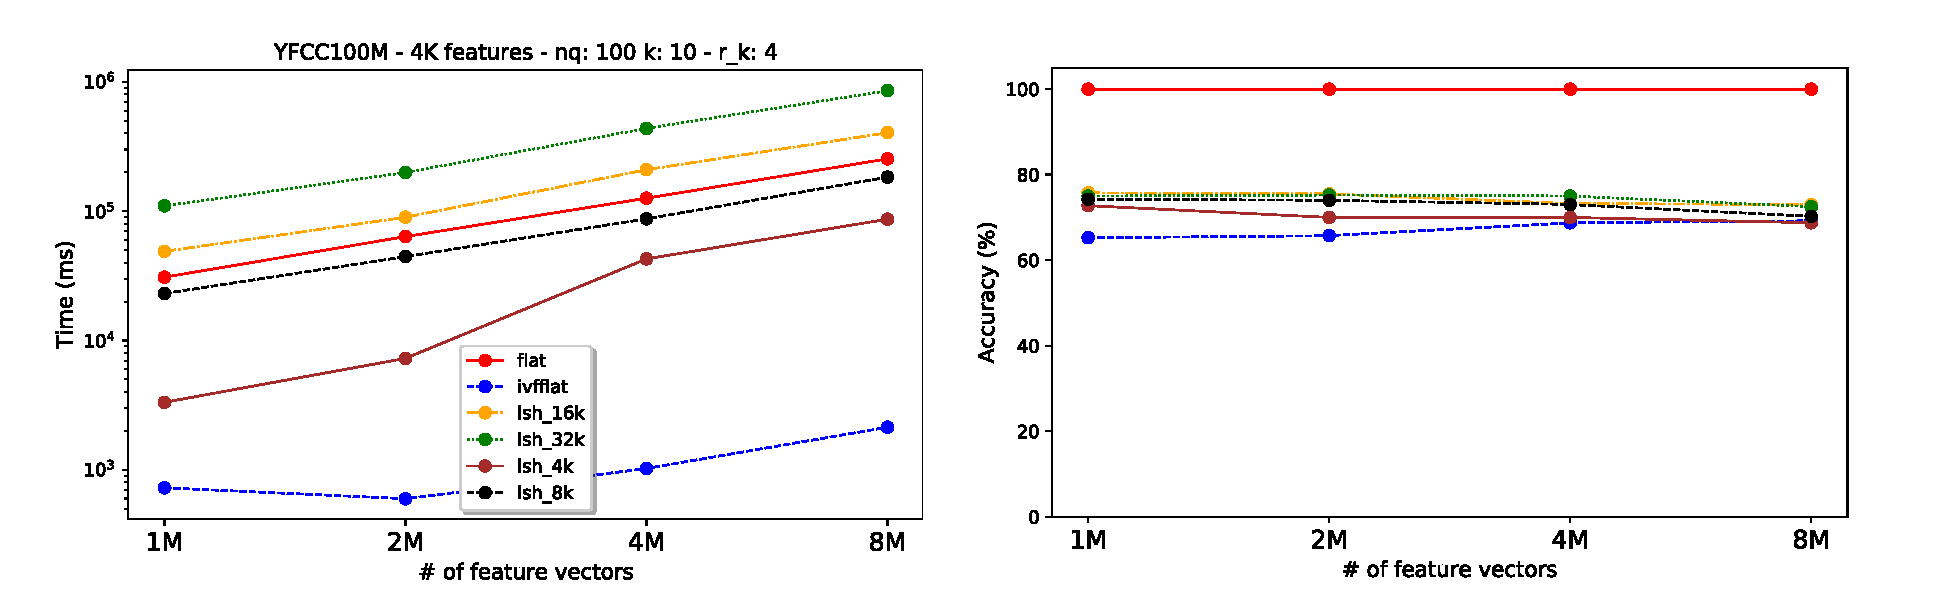
\includegraphics[width=\textwidth]{figures/features_alternatives}
\caption{Feature Vector Evaluation}
\label{fig:features_eval}
\end{figure*}

\begin{figure*}[]
\centering
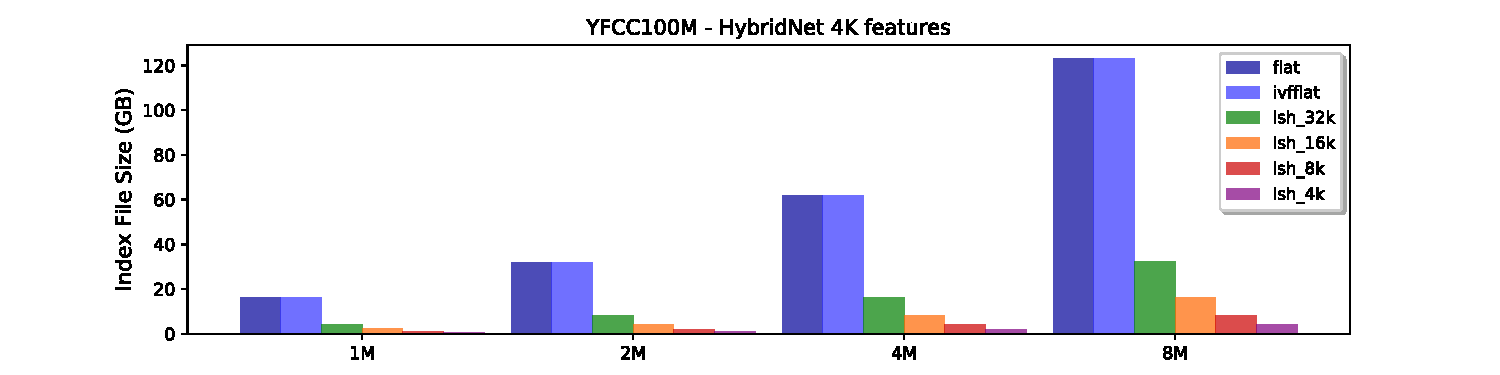
\includegraphics[width=\textwidth]{figures/features_disksize}
\caption{Feature Collection Size in Disk}
\label{fig:features_size_does_matter}
\end{figure*}
